\chapter{METODE PENELITIAN}
\label{chap:desainimplementasi}

% Ubah bagian-bagian berikut dengan isi dari desain dan implementasi

Tugas akhir ini merupakan peelitian pada bidang visi computer yang bertujuan untuk mengendalikan robot menggunakan metode klasifikasi CNN. Secara umum metode yang digunakan adalah pertama pembuatan dataset, prediksi pose tangan, klasifikasi menggunakan model CNN, dan terakhir navigasi control pada robot. Alur metodologi dapat dilihat pada

\begin{figure}[!h]
  \centering
	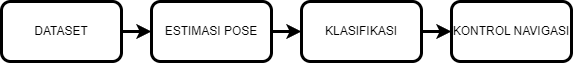
\includegraphics[width=1\linewidth]{../Gambar/metodologi.png}
	\caption{Blok diagram metodologi}
	\label{fig:metodologi}
\end{figure}

\section{Dataset}
\label{sec:deskripsisistem}

Tahapan pengambilan dataset dilakukan dengan mengambilan data-data berupa citra menggunakan kamera pada laptop. Kamera pada laptop dipakai untuk mendapatkan citra yang nantinya digunakan untuk mendeteksi suatu pose atau gestur tangan membutuhkan citra tangan untuk menemukan bagian tangan. Proses pengumpulan citra pose tangan yang digunakan sebagai navigasi robot  dimulai dengan menentukan jumlah kelas dataset. Kelas dataset berjumlah enam pose yang terdiri dari perintah maju, mundur, diam, belok kiri, belok kanan,dan tembak. Setiap pose membutuhkan dua tangan untuk memberikan perintah dengan telapak tangan dihadapkan ke arah kamera. Pose untuk perintah maju dilambangkan dengan kedua tangan mengepal. Pose mundur dilambangkan dengan meluruskan jari manis dan jari tengah seperti halnya pose angka dua pada SIBI pada kedua tangan dan telapak tangan.  Pose diam dilambangkan dengan membuka telapak tangan atau meluruskan semua jari pada kedua tangan.  Pose belok kiri dilambangkan dengan membuka telapak tangan pada tangan kiri dan mengepalkan tangan pada tangan kanan. Pose belok kanan merupakan kebalikan dari pose belok kiri yang dilambangkan dengan tangan kiri mengepal dan tangan kanan membuka telapak tangan. Pose tembak dilambangkan dengan meluruskan ibu jari dan jari manis sedangkan jari lain dikepalkan dengan jari manis diarahkan ke atas dan telapak tangan menghadap ke kamera.

\section{Estimasi Pose}
Pada tahapan ini akan dilakukan deteksi tangan dan ekstraksi fitur. Deteksi tangan akan menggunakan bantuan bantuan \emph{framework Mediapipe}. \emph{Framework Mediapipe} ini memiliki 21 titik  \emph{keypoint} pada tangan. Proses mendeteksi tangan dimulai dengan cara mencari telapak tangan yang terdapat titik nol \emph{keypoint} yang disebut sebagai palm detection model. Setelah titik nol terdeteksi atau telapak tangan ditemukan kemudian mencari 20 titik lainnya pada tangan. Titik-titik \emph{keypoint} ini dicari menggunakan regresi. Setelah 21 titik \emph{keypoint} terdeteksi selanjutnya menyimpan koordinat x dan y relatif terhadap layar yang serta menghubungkan 21 titik tersebut sehingga membentuk \emph{hand landmark} seperti pada Gambar \ref{fig:tangan}. Selanjutnya dilakukan ekstraksi fitur dari \emph{hand landmark} yang telah dibuat. Ekstraksi fitur dilakukan untuk mengurangi \emph{noise} yang terdapat pada citra dataset. Ekstraksi fitur dilakukan dengan menggambar ulang citra \emph{hand landmark} yang telah dibuat oleh \emph{Mediapipe} kedalam citra dengan latar gelap yang selanjutnya akan disebut sebagai citra ekstrasi fitur. Setelah \emph{hand landmark} digambar ulang pada citra dengan latar belakang gelap maka selanjutnya \emph{hand landmark} tiap tangan yang terdeteksi memiliki nilai-nilai koordinat pada tiap \emph{hand landmark}, dari koordinat ini dicari nilai terkecil dan nilai terbesar.  Nilai-nilai ini digunakan untuk membuat \emph{bounding box} pada setiap frame yang terdeteksi tangan didalamnya seperti pada Gambar \ref{fig:boundingbox}. Setiap frame memiliki dua \emph{bounding box} dikarenakan harus terdapat dua tangan untuk bisa mengontrol robot. \emph{Bounding box} dibuat pada citra ekstraksi fitur dengan tujuan untuk menormalisasi posisi. Normalisasi posisi dilakukan dengan hanya menyimpan citra didalam bounding box dengan cara membuang citra diluar bounding box. Setelah citra yang tersisa hanya didalam bounding box, selanjunya kedua bounding box tersebut akan di susun secara horizontal. Penyusunan ini dikarenakan pada citra ekstraksi fitur terdapat 2 \emph{hand landmark}. Setelah disusun citra ekstraksi akan disimpan sebagai data pada saat klasifikasi.

\begin{figure}
  \centering
  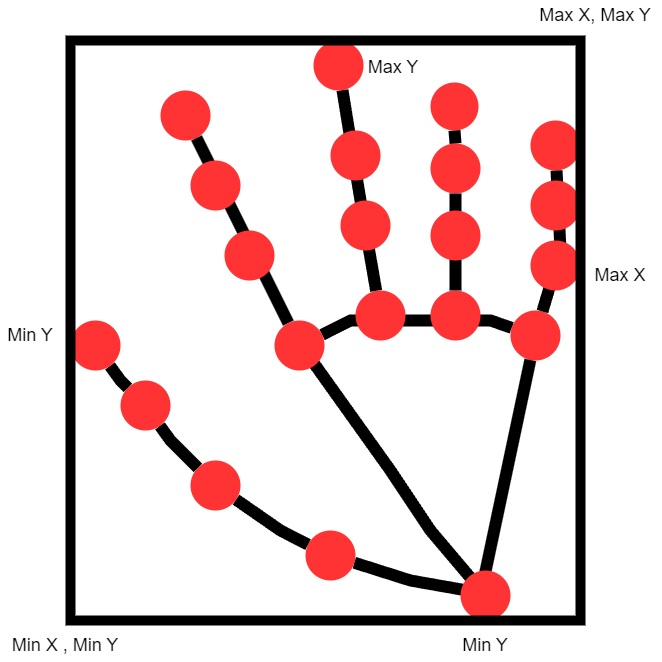
\includegraphics[width=0.5\linewidth]{../Gambar/boundingbox.png}
  \caption{\emph{Bounding Box}}
  \label{fig:boundingbox}
\end{figure}

\section{Klasifikasi}

\begin{figure}[!h]
  \centering
  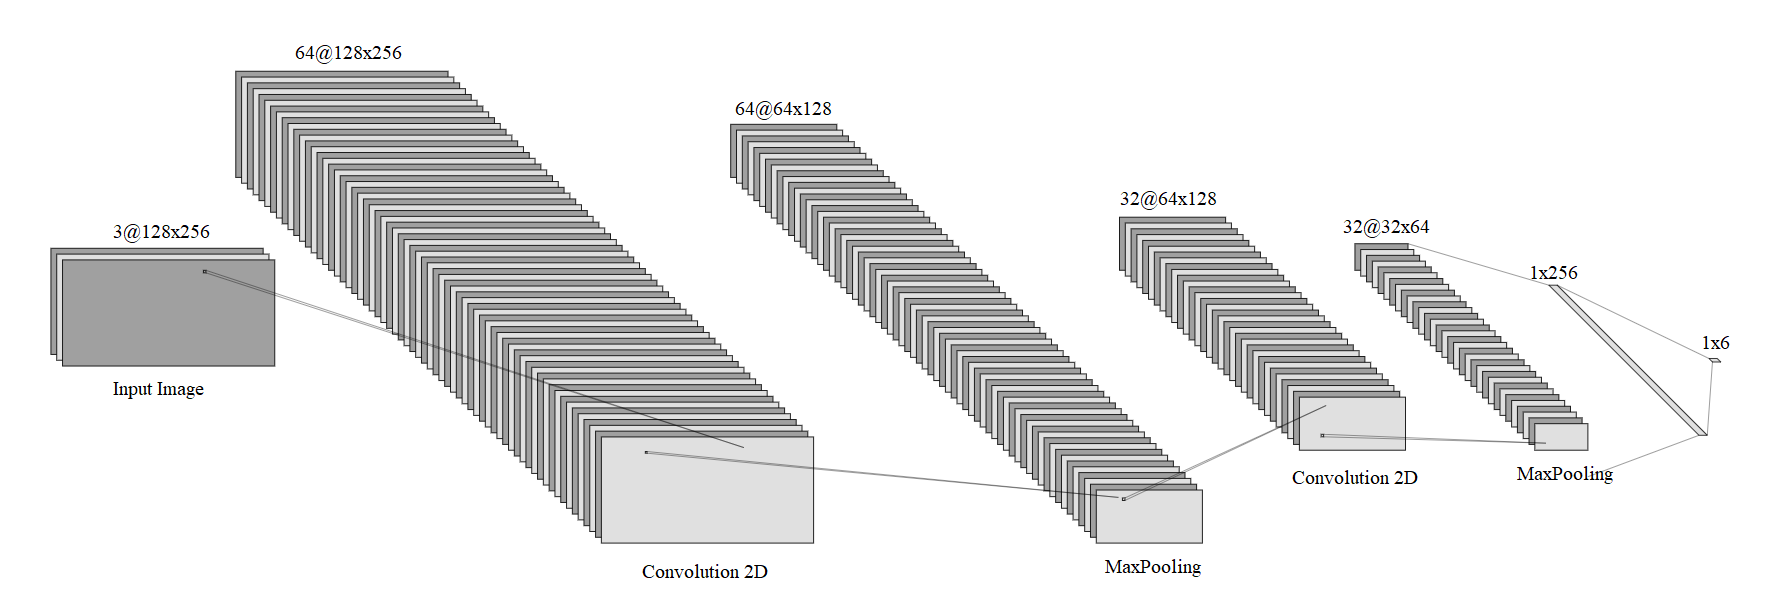
\includegraphics[width=1\linewidth]{../Gambar/LayerCnn.png}
  \caption{Layer CNN}
  \label{fig:layerCNn}
\end{figure}

Sebelum dilakukannya klasifikasi dilakukan \emph{training} data terlebih dahulu. \emph{Training} data merupakan tahapan dari dataset yang telah dibuat yang kemudian dilatih untuk memperoleh suatu pola dari data tersebut. Pola tersebut digunakan untuk membantu mengenali objek dalam citra. Dalam proses \emph{training} dibutuhkan konfigurasi yang digunakan. Konfigurasi \emph{training} yang digunakan yaitu CNN dengan layer \emph{layer convolution}, \emph{layer max pooling},  dan flatten seperti yang ditampilkan pada Gambar \ref*{fig:layerCNn}. Adapun layer-layer tersebut membutuhkan konfigurasi seperti berikut :
\begin{enumerate}
  \item \emph{Convolution Layer}. \emph{Convolution layer} merupakan layer pertama dalam CNN yang melakukan proses konvolusi pada data citra untuk mengekstraksi fitur dari citra input sesuai dengan banyaknya filter yang digunakan \parencite{konvolusilayer}. 
  \item \emph{Pooling Layer}. \emph{Pooling layer} merupakan metode \emph{down-sumpling} yang bertujuan untuk mengurangi kompleksitas pada \emph{layer} selanjutnya. Pada penelitian ini akan dilakukan dengan metode max pooling yaitu mengambil nilai maksimal dari data citra dan bergerak dengan pergeseran \emph{layer} \parencite{poolilayer}.
  \item \emph{Fully-Connected Layer}. \emph{Fully-Connected layer} merupakan \emph{layer} yang digunakan untuk mengubah multidimensi data menjadi satu dimensi atau vektor. Layer ini digunakan setelah layer konvolusi dan pooling telah dilaksanakan. Cara kerja dari \emph{Fully-Connected layer} adalah memberikan nilai perkalian acak dari bobot dan bias \parencite{flayenlayer}
\end{enumerate}
Sebelum dilakukan proses \emph{train} menggunakan CNN, perlu dilakukan beberapa konfigurasi pada \emph{hyperparameter}. Adapun konfigurasi \emph{hyperparameter} yang dilakukan pada CNN untuk \emph{train} dataset yaitu :
\begin{enumerate}
  \item \emph{Epochs}. \emph{Epochs} merupakan hyperparameter yang digunakan untuk menentuan jumlah pengulangan suatu algoritma learning pada suatu training dataset. Semakin besar jumlah \emph{epoch} maka akan membutuhkan waktu yang lama dalam melakukan training dataset, namun semakin banyak \emph{epoch} dapat meningkatkan akurasi pada model yang dihasilkan.
  \item \emph{Batch-Size}. \emph{Batchsize} merupakan hyperparameter yang digunakan untuk mengatue jumlah sampel yraing yang dikerjakan sebelum parameter model diperbarui.
  \item \emph{Image Size}. \emph{Image Size} adalah ukuran dari citra dari dataset. Semakin besar suatu ukuran citra maka semakin lama waktu yang dibutuhkan untuk training semakin lama.
  \item \emph{Optimizer}. \emph{Optimizer} merupakan metode yang digunakan untuk meminimalisir eror. \emph{Optimizer} merupakan fungsi matematika yang bergantung pada parameter model yang dapat dipelajari seperti weight dan bias. \emph{Optimizer} berguna untuk mengetahui cara memodifikasi weight dan learning rate untuk mengurangi loss \parencite{optimizer}.
\end{enumerate} 
Setelah dilakukan proses \emph{validation} dan model yang telah dibuat memiliki akurasi yang tinggi (sesuai dengan \emph{threshold}), maka tahapan selanjutnya yaitu klasifikasi. Tahap klasifikasi dilakukan dengan menginputkan dataset baru melalu kamera. Model yang telah dibuat akan menerima citra dataset serta dikenali posenya. Pose yang posenya telah diketahui selanjutnya diterjemahkan menjadi kode instruksi yang menjadi acuan dalam memberikan perintah kepada robot.


\section{Kontrol Navigasi} 
Tahapan ini berupa cara mengontrol robot menggunakan kode intruksi dari hasil klasifikasi. Laptop dengan robot terhubung secara \emph{wireless} menggunakan koneksi internet. Hasil klasifikasi dari laptop dikirimkan kepada robot menggunakan jaringan Websocket, dimana laptop dan robot terhubung dalam suatu port dan ip yang telah ditentukan. Websocket merupakan protokol pada \emph{layer} aplikasi dalam \emph{osi layer}. Pada Websocket memungkingkan koneksi dua arah antara client dan server dengan membangun satu buah jalur komunikasi \parencite{websocket}. Perancangan pada robot dibuat dengan kemampuan yang dapat dilakukan oleh robot. Kebutuhan pada kemampuan robot yaitu menggerakkan seluruh badan robot dan menembak serta komunikasi dengan internet. Robot dapat dikontrol sesuai dari banyaknya \emph{class} pada model yang telah dibuat dalam hal ini terdapat enam \emph{class}. Aksi dari robot ini sesuai dari data yang diterima dari hasil klasifikasi yakni maju, mundur, kanan, kiri, diam, dan tembak. Tiap-tiap aksi diwakilkan dengan huruf abjad tertentu. Sesuai dengan aksi-aksi tersebut maka pergerakan robot dapat terjadi dikarenakan adanya sepasang roda yang dipasangkan pada robot. Perputaran roda diatur dari motor driver dengan menyalurkan listrik kepada motor dc yang sudah dipasangkan roda sebagai outputya. Kemampuan robot untuk tembak menembak menggunakan bantuan \emph{infrared}. Tiap robot memiliki \emph{infrared} \emph{transmitter} dan \emph{infrared} \emph{receiver} yang diletakkan disekeliling robot. Aksi menembak dimulai dari \emph{infrared} \emph{transmitter} mengirimkan pesan dan diterima oleh \emph{infrared} \emph{receiver}. Rancangan desain robot dapat dilihat pada Gambar \ref{fig:rancanganrobot}

\begin{figure}[!h]
  \centering
  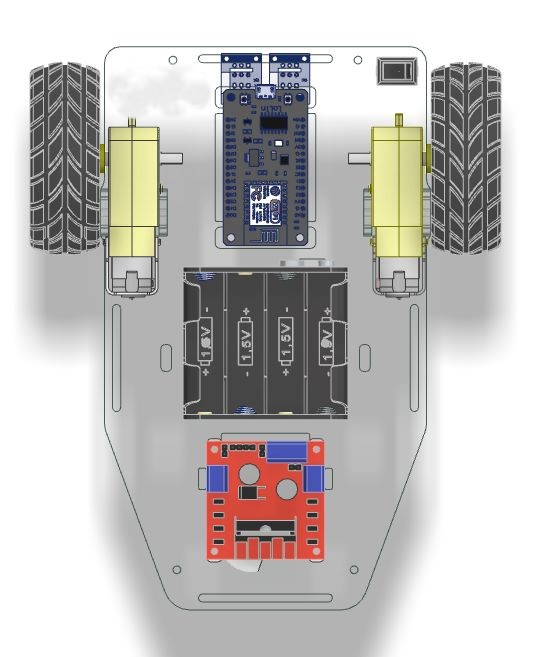
\includegraphics[width=0.3\linewidth]{../Gambar/rancnaganrobot.jpg}
  \caption{Rancangan desain robot}
  \label{fig:rancanganrobot}
\end{figure}
